
\subsection{Answers}
\begin{table}[htb]%
\begin{center}%
\caption{Q7: Which fields are you mostly working in?}%
\label{tab:Q7-ans}%
\begin{tabular}{l|l|r}%
\hline%
Choice & Abbrv. & \# Answers \\%
\hline%
Numerical application and/or library & Num-Lib. & 611 (72.1\%) \\%
{\small Parallel language (incl. domain specific$\cdots$} & Lang & 165 (19.5\%) \\%
{\small System software development (OS, runtime$\cdots$} & OS/R & 155 (18.3\%) \\%
{\small Tool development (performance tuning, de$\cdots$} & Tool & 127 (15.0\%) \\%
Big data & Big data & 87 (10.3\%) \\%
Visualization & Vis. & 77 (9.1\%) \\%
AI (Deep Learning) & AI & 66 (7.8\%) \\%
Workflow and/or In-situ & Worlflow & 50 (5.9\%) \\%
Image processing & Image & 43 (5.1\%) \\%
other & - & 70 (8.3\%) \\%
\hline%
\multicolumn{2}{c}{total} & 1451 (848)\\%
\hline%
\end{tabular}%
\end{center}%
\end{table}%


42\% responded from persons working with the
numerical application and library. This indicates that most of the
respondents 
are developing parallel application and library using MPI. Hence they
are at the top of 
the software stack. People working at the intermediate layers if the
stack (runtime, language , workflow, etc.) account for 39\%. Other 
application domains (Big data, AI, image, etc. ) account for 14\%. 

\mycomment[AH]{I supposed to have more people are working for Big Data
  and AI, but this result shows the traditional numerical apps
  dominates. Hmmm, what was the fuss of Biga Data and AI and where do
  they go? One possibility of this is that this survey failed to reach
them. What is the truth?}

\subsection{List of other answers}
\begin{itemize}
\item Central and South America: I/O
\item China: Computational Fluid Dynamics
\item China: Computational fluid dynamics
\item China: other
\item Europe:France: Astronomical simulations
\item Europe:France: Bioinformatics
\item Europe:France: C.F.D.
\item Europe:France: Computational fluid dynamics
\item Europe:France: Physics
\item Europe:France: Storage systems
\item Europe:France: cryptanalysis
\item Europe:France: statistics
\item Europe:Germany: Algorithms
\item Europe:Germany: Cloud
\item Europe:Germany: Computational science
\item Europe:Germany: Earth System Science
\item Europe:Germany: Peformance analysis
\item Europe:Germany: Research applications
\item Europe:Germany: Simulation
\item Europe:Germany: Teaching of MPI and OpenMP
\item Europe:Germany: administration, workflow management / counseling
\item Europe:Germany: data analysis from CFD
\item Europe:Germany: research
\item Europe:Italy: Scientific simulations
\item Europe:Italy: Scientific software, Molecular Dynamics, Monte Carlo
\item Europe:Italy: Theoretical nuclear physics
\item Europe:Italy: scientific software development
\item Europe:Italy: three-dimensional magnetohydrodynamic parallel codes
\item Europe:UK: Application optimisation and benchmarking
\item Europe:UK: Applications
\item Europe:UK: Plasma Physics
\item Europe:UK: Plasma Physics
\item Europe:UK: Research software development
\item Europe:UK: Scientific research
\item Europe:UK: Scientific software
\item Europe:UK: claiClimate and Weather simulation (probably numerical application then)
\item Europe:others: Algorithms
\item Europe:others: Astrophysics
\item Europe:others: Bioinformatics
\item Europe:others: Bioinformatics
\item Europe:others: Lattice Field Theory
\item Europe:others: Performance analysis
\item Europe:others: Scientific calculations
\item Europe:others: Simulation
\item Europe:others: Theoretical/computational condensed matter physics
\item Europe:others: biophysics simluation software
\item Europe:others: computational physics
\item Europe:others: material science simulation
\item Europe:others: scientific software
\item Europe:others: thermal physics and fluiddynamics
\item India: Bioinformatics Applications
\item Japan: AI (non deep learning)
\item Japan: Bioinformatics
\item Japan: Fluid Mechanics
\item Japan: Microarchitecture
\item Japan: Scientific software
\item Japan: Super computer system operation
\item Russia: High-performance simulations in applied science
\item Russia: Life Science, Biochemistry
\item Russia: Scientific computing
\item Russia: fault tolerance of parallel computation
\item Russia: information structure analysis
\item Russia: machine learning
\item Russia: plasma simulations
\item Russia: science modeling
\item Russia: scientific research
\item South Korea: Atmospheric circulation modeling
\item South Korea: cfd
\item USA: Neuroscience modelling
\item USA: implementing parallel codes, performance optimization

\end{itemize}

\begin{figure}[htb]
\begin{center}
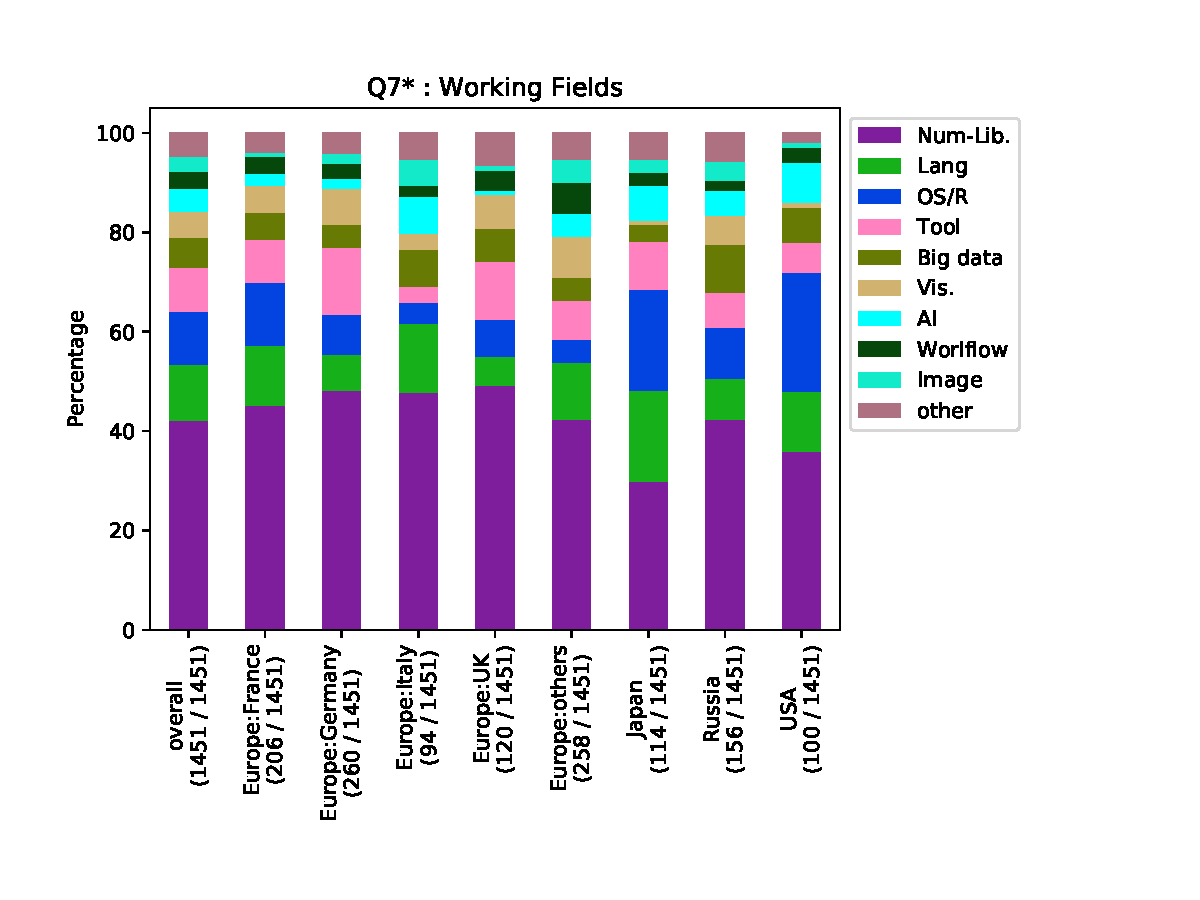
\includegraphics[width=10cm]{../pdfs/Q7.pdf}
\caption{Simple analysis: Q7}
\label{fig:Q7}
\end{center}
\end{figure}
